\documentclass[twoside]{article}

% Packages required by doxygen
\usepackage{fixltx2e}
\usepackage{calc}
\usepackage{doxygen}
\usepackage{graphicx}
\usepackage[utf8]{inputenc}
\usepackage{makeidx}
\usepackage{multicol}
\usepackage{multirow}
\PassOptionsToPackage{warn}{textcomp}
\usepackage{textcomp}
\usepackage[nointegrals]{wasysym}
\usepackage[table]{xcolor}

% Font selection
\usepackage[T1]{fontenc}
\usepackage{mathptmx}
\usepackage[scaled=.90]{helvet}
\usepackage{courier}
\usepackage{amssymb}
\usepackage{sectsty}
\renewcommand{\familydefault}{\sfdefault}
\allsectionsfont{%
  \fontseries{bc}\selectfont%
  \color{darkgray}%
}
\renewcommand{\DoxyLabelFont}{%
  \fontseries{bc}\selectfont%
  \color{darkgray}%
}
\newcommand{\+}{\discretionary{\mbox{\scriptsize$\hookleftarrow$}}{}{}}

% Page & text layout
\usepackage[screen]{geometry}
\tolerance=750
\hfuzz=15pt
\hbadness=750
\setlength{\emergencystretch}{15pt}
\setlength{\parindent}{0cm}
\setlength{\parskip}{0.2cm}
\makeatletter
\renewcommand{\paragraph}{%
  \@startsection{paragraph}{4}{0ex}{-1.0ex}{1.0ex}{%
    \normalfont\normalsize\bfseries\SS@parafont%
  }%
}
\renewcommand{\subparagraph}{%
  \@startsection{subparagraph}{5}{0ex}{-1.0ex}{1.0ex}{%
    \normalfont\normalsize\bfseries\SS@subparafont%
  }%
}
\makeatother

% Headers & footers
\usepackage{fancyhdr}
\pagestyle{fancyplain}
\fancyhead[LE]{\fancyplain{}{\bfseries\thepage}}
\fancyhead[CE]{\fancyplain{}{}}
\fancyhead[RE]{\fancyplain{}{\bfseries\leftmark}}
\fancyhead[LO]{\fancyplain{}{\bfseries\rightmark}}
\fancyhead[CO]{\fancyplain{}{}}
\fancyhead[RO]{\fancyplain{}{\bfseries\thepage}}
\fancyfoot[LE]{\fancyplain{}{}}
\fancyfoot[CE]{\fancyplain{}{}}
\fancyfoot[RE]{\fancyplain{}{\bfseries\scriptsize Generated on Thu Nov 16 2017 15\+:56\+:08 for Lab6\+Morse\+Code\+Lab by Doxygen }}
\fancyfoot[LO]{\fancyplain{}{\bfseries\scriptsize Generated on Thu Nov 16 2017 15\+:56\+:08 for Lab6\+Morse\+Code\+Lab by Doxygen }}
\fancyfoot[CO]{\fancyplain{}{}}
\fancyfoot[RO]{\fancyplain{}{}}
\renewcommand{\footrulewidth}{0.4pt}
\renewcommand{\sectionmark}[1]{%
  \markright{\thesection\ #1}%
}

% Indices & bibliography
\usepackage{natbib}
\usepackage[titles]{tocloft}
\setcounter{tocdepth}{3}
\setcounter{secnumdepth}{5}
\makeindex

% Packages requested by user
\usepackage{titlesec}

% Hyperlinks (required, but should be loaded last)
\usepackage{ifpdf}
\ifpdf
  \usepackage[pdftex,pagebackref=true]{hyperref}
\else
  \usepackage[ps2pdf,pagebackref=true]{hyperref}
\fi
\hypersetup{%
  colorlinks=true,%
  linkcolor=blue,%
  citecolor=blue,%
  unicode%
}

% Custom commands
\newcommand{\clearemptydoublepage}{%
  \newpage{\pagestyle{empty}\cleardoublepage}%
}


\newcommand{\sectionbreak}{\clearpage}

\begin{document}

% Titlepage & ToC
\hypersetup{pageanchor=false,
             bookmarks=true,
             bookmarksnumbered=true,
             pdfencoding=unicode
            }
\pagenumbering{roman}
\begin{titlepage}
\vspace*{7cm}
\begin{center}%
{\Large Lab6\+Morse\+Code\+Lab }\\
\vspace*{1cm}
{\large Generated by Doxygen 1.8.8}\\
\vspace*{0.5cm}
{\small Thu Nov 16 2017 15:56:08}\\
\end{center}
\end{titlepage}
\tableofcontents
\pagenumbering{arabic}
\hypersetup{pageanchor=true}

%--- Begin generated contents ---
\section{Specification}
\label{Specification}
\hypertarget{Specification}{}
This program has a built in dictionary for english that can be translated to tagalog. It has a user input in which the user may add the translation of a word that is not within the dictionary. 
\section{Analysis}
\label{Analysis}
\hypertarget{Analysis}{}
inputs will be\+:

\begin{DoxyItemize}
\item The outputs will be\+:\end{DoxyItemize}
\begin{DoxyItemize}
\item The overall algorithim is\+: \end{DoxyItemize}

\section{Design}
\label{Design}
\hypertarget{Design}{}
When this program is launched, the user is given the option to choose from any company they would like do their stock exchange. They are given five different companies in a drop down bar to choose from. Once the user has chosen a company, they are given the option to either sell or buy. After the user has chosen one of those two options, the user is then, asked to give their name, shares amount, and price. After the user has entered the following, the program will then execute and insert the information into the heap tree and search through the heap tree. The heap tree will try to find a matching price that the user has input and it will execute the purchase. If there was no match, it will output \char`\"{}\+No seller/buyer\char`\"{} for the user. Also, if the user enter's the name market, it will purchase/sell the shares from the market. After every purchase and sell, it will display in the live graph and live table. The graph and table will update after every transaction. 
\section{Testcase1}
\label{Testcase1}
\hypertarget{Testcase1}{}
This is our home html page. Let's try to encode the word \char`\"{}trees\char`\"{}. After we hit the go button, we should be redirected to a new html page with \char`\"{}trees\char`\"{} translated to morse code.

 
    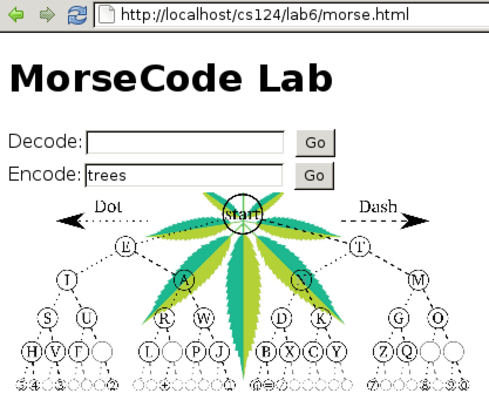
\includegraphics{../test21.png}
     
\section{Testcase2}
\label{Testcase2}
\hypertarget{Testcase2}{}
Nice it worked. Now let's copy the output from our morse code and validate it using our decode function.

 
    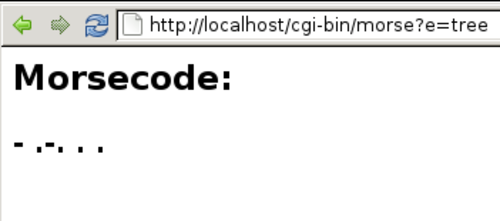
\includegraphics{../test31.png}
     
\section{Testcase3}
\label{Testcase3}
\hypertarget{Testcase3}{}
After copying pasting into our decode text field. We should get an abc translation when we click the go button.

 
    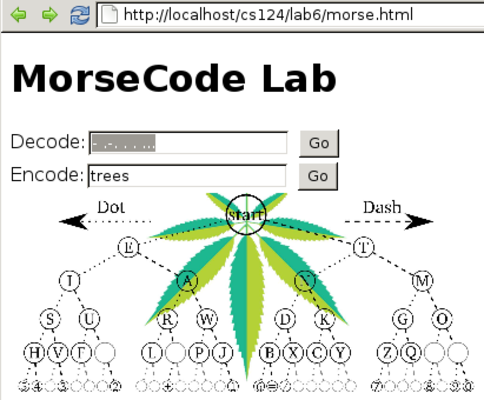
\includegraphics{../test41.png}
     
\section{Testcase4}
\label{Testcase4}
\hypertarget{Testcase4}{}
Great! Our encode function works and our decode function work since our inputs match the outputs.

 
    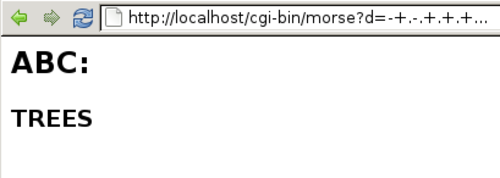
\includegraphics{../test51.png}
     
\section{Testcase5}
\label{Testcase5}
\hypertarget{Testcase5}{}
Now let's try another test. Let's encode \char`\"{}\+Topham\char`\"{}. We should receive the morsecode translation of it.

 
    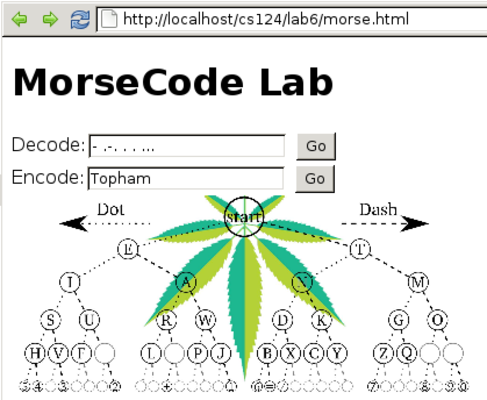
\includegraphics{../test61.png}
     
\section{Testcase6}
\label{Testcase6}
\hypertarget{Testcase6}{}
Awesome! let's copy and paste this morsecode in to our decode function to validate it.

 
    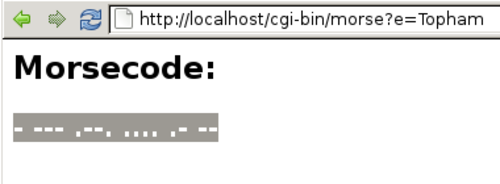
\includegraphics{../test71.png}
     
\section{Testcase7}
\label{Testcase7}
\hypertarget{Testcase7}{}
We should see \char`\"{}\+T\+O\+P\+H\+A\+M\char`\"{} when we submit it.  
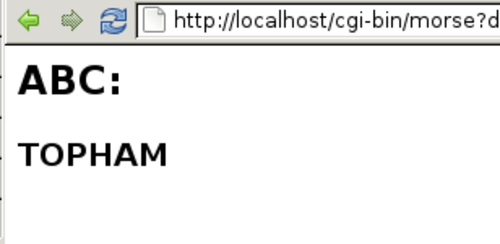
\includegraphics{../test81.png}
 
\section{Testcase8}
\label{Testcase8}
\hypertarget{Testcase8}{}
Beautiful. Let's try one more test case to make sure it works.

 
    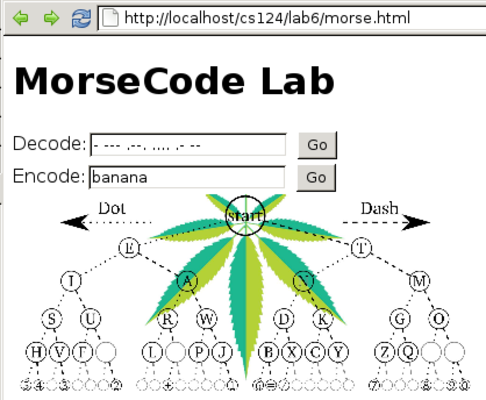
\includegraphics{../test91.png}
     
\section{Testcase9}
\label{Testcase9}
\hypertarget{Testcase9}{}
Here we try our favorite word \char`\"{}banana\char`\"{}.

 
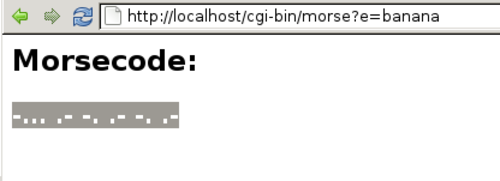
\includegraphics{../test101.png}
 
\section{Testcase10}
\label{Testcase10}
\hypertarget{Testcase10}{}
 
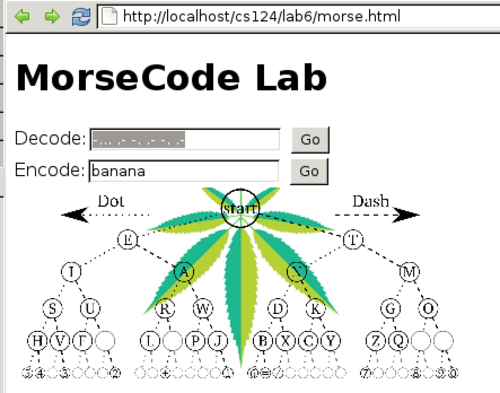
\includegraphics{../test111.png}
 
\section{Testcase11}
\label{Testcase11}
\hypertarget{Testcase11}{}
Great test case 3 works too!

 
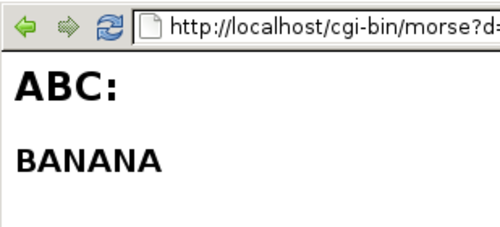
\includegraphics{../test121.png}
 
\section{Testcase12}
\label{Testcase12}
\hypertarget{Testcase12}{}
D\+D\+D Tree Example

 
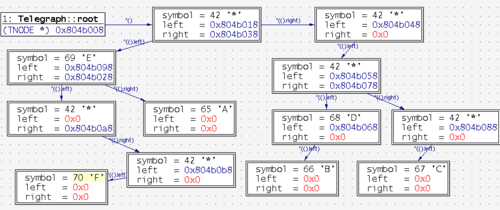
\includegraphics{../dddtree1.png}
 
\section{diagram}
\label{diagram}
\hypertarget{diagram}{}

\begin{DoxyImageNoCaption}
  \mbox{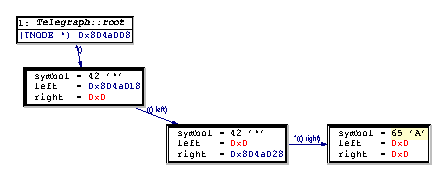
\includegraphics{dddgraph}}
\end{DoxyImageNoCaption}
 
\section{Class Index}
\subsection{Class List}
Here are the classes, structs, unions and interfaces with brief descriptions\+:\begin{DoxyCompactList}
\item\contentsline{section}{\hyperlink{structENTRY}{E\+N\+T\+R\+Y} }{\pageref{structENTRY}}{}
\end{DoxyCompactList}

\section{File Index}
\subsection{File List}
Here is a list of all files with brief descriptions\+:\begin{DoxyCompactList}
\item\contentsline{section}{\hyperlink{BuildListDirectly_8cpp}{Build\+List\+Directly.\+cpp} }{\pageref{BuildListDirectly_8cpp}}{}
\item\contentsline{section}{\hyperlink{destroyList_8cpp}{destroy\+List.\+cpp} }{\pageref{destroyList_8cpp}}{}
\item\contentsline{section}{\hyperlink{displayList_8cpp}{display\+List.\+cpp} }{\pageref{displayList_8cpp}}{}
\item\contentsline{section}{\hyperlink{Insert_8cpp}{Insert.\+cpp} }{\pageref{Insert_8cpp}}{}
\item\contentsline{section}{\hyperlink{InsertInOrder_8cpp}{Insert\+In\+Order.\+cpp} }{\pageref{InsertInOrder_8cpp}}{}
\item\contentsline{section}{\hyperlink{lab2_8h}{lab2.\+h} }{\pageref{lab2_8h}}{}
\item\contentsline{section}{\hyperlink{loadList_8cpp}{load\+List.\+cpp} }{\pageref{loadList_8cpp}}{}
\item\contentsline{section}{\hyperlink{loadList2_8cpp}{load\+List2.\+cpp} }{\pageref{loadList2_8cpp}}{}
\item\contentsline{section}{\hyperlink{loadList3_8cpp}{load\+List3.\+cpp} }{\pageref{loadList3_8cpp}}{}
\item\contentsline{section}{\hyperlink{main_8cpp}{main.\+cpp} }{\pageref{main_8cpp}}{}
\end{DoxyCompactList}

\section{Class Documentation}
\hypertarget{structMorsecode}{\subsection{Morsecode Struct Reference}
\label{structMorsecode}\index{Morsecode@{Morsecode}}
}


{\ttfamily \#include $<$morse.\+h$>$}

\subsubsection*{Public Types}
\begin{DoxyCompactItemize}
\item 
enum \{ \hyperlink{structMorsecode_ad8b781b4f5aa87b0afdef835324bcf24a352dad4a744b50bf7d7db44a4959260f}{N} =7
 \}
\end{DoxyCompactItemize}
\subsubsection*{Public Attributes}
\begin{DoxyCompactItemize}
\item 
char \hyperlink{structMorsecode_a8f7fb86f9de77dc705dc37730e83869b}{symbol}
\item 
char \hyperlink{structMorsecode_abb81632acf39b9e91f76bd09b12fc0e0}{code} \mbox{[}\hyperlink{structMorsecode_ad8b781b4f5aa87b0afdef835324bcf24a352dad4a744b50bf7d7db44a4959260f}{N}\mbox{]}
\end{DoxyCompactItemize}


\subsubsection{Member Enumeration Documentation}
\hypertarget{structMorsecode_ad8b781b4f5aa87b0afdef835324bcf24}{\paragraph[{anonymous enum}]{\setlength{\rightskip}{0pt plus 5cm}anonymous enum}}\label{structMorsecode_ad8b781b4f5aa87b0afdef835324bcf24}
\begin{Desc}
\item[Enumerator]\par
\begin{description}
\index{N@{N}!Morsecode@{Morsecode}}\index{Morsecode@{Morsecode}!N@{N}}\item[{\em 
\hypertarget{structMorsecode_ad8b781b4f5aa87b0afdef835324bcf24a352dad4a744b50bf7d7db44a4959260f}{N}\label{structMorsecode_ad8b781b4f5aa87b0afdef835324bcf24a352dad4a744b50bf7d7db44a4959260f}
}]\end{description}
\end{Desc}

\begin{DoxyCode}
7 \{\hyperlink{structMorsecode_ad8b781b4f5aa87b0afdef835324bcf24a352dad4a744b50bf7d7db44a4959260f}{N}=7\};
\end{DoxyCode}


\subsubsection{Member Data Documentation}
\hypertarget{structMorsecode_abb81632acf39b9e91f76bd09b12fc0e0}{\index{Morsecode@{Morsecode}!code@{code}}
\index{code@{code}!Morsecode@{Morsecode}}
\paragraph[{code}]{\setlength{\rightskip}{0pt plus 5cm}char Morsecode\+::code\mbox{[}{\bf N}\mbox{]}}}\label{structMorsecode_abb81632acf39b9e91f76bd09b12fc0e0}
\hypertarget{structMorsecode_a8f7fb86f9de77dc705dc37730e83869b}{\index{Morsecode@{Morsecode}!symbol@{symbol}}
\index{symbol@{symbol}!Morsecode@{Morsecode}}
\paragraph[{symbol}]{\setlength{\rightskip}{0pt plus 5cm}char Morsecode\+::symbol}}\label{structMorsecode_a8f7fb86f9de77dc705dc37730e83869b}


The documentation for this struct was generated from the following file\+:\begin{DoxyCompactItemize}
\item 
\hyperlink{morse_8h}{morse.\+h}\end{DoxyCompactItemize}

\hypertarget{classTelegraph}{\subsection{Telegraph Class Reference}
\label{classTelegraph}\index{Telegraph@{Telegraph}}
}


{\ttfamily \#include $<$morse.\+h$>$}

\subsubsection*{Public Member Functions}
\begin{DoxyCompactItemize}
\item 
void \hyperlink{classTelegraph_a73c4f9c8862ba581ec5eac6530bf6352}{Encode} (char text\mbox{[}$\,$\mbox{]}, char morse\mbox{[}$\,$\mbox{]})
\item 
void \hyperlink{classTelegraph_a09985235f674760465da3bbd9e136d12}{Decode} (char morse\mbox{[}$\,$\mbox{]}, char text\mbox{[}$\,$\mbox{]})
\end{DoxyCompactItemize}
\subsubsection*{Static Public Member Functions}
\begin{DoxyCompactItemize}
\item 
static void \hyperlink{classTelegraph_a2ace7d6ba4d3742dbcc57d6a36a13b54}{open} ()
\begin{DoxyCompactList}\small\item\em open creates the morse code table \end{DoxyCompactList}\item 
static void \hyperlink{classTelegraph_a4b7e7f129e6aedc1c3f9b354806f265e}{close} ()
\item 
static void \hyperlink{classTelegraph_ae7f12363fff79578576b345c9d8cb8fb}{destroy\+Tree} ()
\end{DoxyCompactItemize}


\subsubsection{Member Function Documentation}
\hypertarget{classTelegraph_a4b7e7f129e6aedc1c3f9b354806f265e}{\index{Telegraph@{Telegraph}!close@{close}}
\index{close@{close}!Telegraph@{Telegraph}}
\paragraph[{close}]{\setlength{\rightskip}{0pt plus 5cm}void Telegraph\+::close (
\begin{DoxyParamCaption}
{}
\end{DoxyParamCaption}
)\hspace{0.3cm}{\ttfamily [static]}}}\label{classTelegraph_a4b7e7f129e6aedc1c3f9b354806f265e}

\begin{DoxyCode}
68 \{
69     \hyperlink{classTelegraph_ae7f12363fff79578576b345c9d8cb8fb}{destroyTree}(root);
70     root = 0;
71 \}
\end{DoxyCode}
\hypertarget{classTelegraph_a09985235f674760465da3bbd9e136d12}{\index{Telegraph@{Telegraph}!Decode@{Decode}}
\index{Decode@{Decode}!Telegraph@{Telegraph}}
\paragraph[{Decode}]{\setlength{\rightskip}{0pt plus 5cm}void Telegraph\+::\+Decode (
\begin{DoxyParamCaption}
\item[{char}]{morse\mbox{[}$\,$\mbox{]}, }
\item[{char}]{text\mbox{[}$\,$\mbox{]}}
\end{DoxyParamCaption}
)}}\label{classTelegraph_a09985235f674760465da3bbd9e136d12}

\begin{DoxyCode}
101 \{
102      \textcolor{keywordtype}{char} *dd;
103      \hyperlink{structTNODE}{TNODE} *node;
104      node = root;
105      \textcolor{comment}{//char *t;}
106      \textcolor{comment}{// For each char in the encoded message (can be}
107      \textcolor{comment}{// a dot, a dash, or a space):}
108      \textcolor{keywordflow}{for} (dd = morse; *dd; dd++) \{
109         \textcolor{keywordflow}{if}(*dd == \textcolor{charliteral}{'.'})
110             node = node->\hyperlink{structTNODE_ac8548d0ee2d54b914e0e07ab35375dba}{left};
111         \textcolor{keywordflow}{else} \textcolor{keywordflow}{if}(*dd == \textcolor{charliteral}{'-'})
112             node = node->\hyperlink{structTNODE_a4e135d9137519b2a4b89dbccb55ae967}{right}; 
113         \textcolor{keywordflow}{else} \{
114             *text++ = node->\hyperlink{structTNODE_a436db20d992c4227b8482603b4f76712}{symbol}; 
115             node = root;
116         \}
117      \}
118      *text = \textcolor{charliteral}{'\(\backslash\)0'};
119 \}
\end{DoxyCode}
\hypertarget{classTelegraph_ae7f12363fff79578576b345c9d8cb8fb}{\index{Telegraph@{Telegraph}!destroy\+Tree@{destroy\+Tree}}
\index{destroy\+Tree@{destroy\+Tree}!Telegraph@{Telegraph}}
\paragraph[{destroy\+Tree}]{\setlength{\rightskip}{0pt plus 5cm}static void Telegraph\+::destroy\+Tree (
\begin{DoxyParamCaption}
{}
\end{DoxyParamCaption}
)\hspace{0.3cm}{\ttfamily [static]}}}\label{classTelegraph_ae7f12363fff79578576b345c9d8cb8fb}
\hypertarget{classTelegraph_a73c4f9c8862ba581ec5eac6530bf6352}{\index{Telegraph@{Telegraph}!Encode@{Encode}}
\index{Encode@{Encode}!Telegraph@{Telegraph}}
\paragraph[{Encode}]{\setlength{\rightskip}{0pt plus 5cm}void Telegraph\+::\+Encode (
\begin{DoxyParamCaption}
\item[{char}]{text\mbox{[}$\,$\mbox{]}, }
\item[{char}]{morse\mbox{[}$\,$\mbox{]}}
\end{DoxyParamCaption}
)}}\label{classTelegraph_a73c4f9c8862ba581ec5eac6530bf6352}

\begin{DoxyCode}
75 \{
76      \textcolor{keywordtype}{int} i;
77      \textcolor{keywordtype}{char} c, *t, *dd; \textcolor{comment}{// t points to text;}
78      \textcolor{comment}{// dd points to a string of dots and dashes.}
79      \textcolor{keywordflow}{for} (t = text; *t; t++) \{
80          c = toupper(*t);
81          \textcolor{comment}{// If space, add a space to the morse string:}
82          \textcolor{keywordflow}{if} (c == \textcolor{charliteral}{' '}) \{
83              *morse++ = \textcolor{charliteral}{' '};
84              \textcolor{keywordflow}{continue};
85          \}
86          \textcolor{comment}{// Find this symbol in the MORSECODE table;}
87          \textcolor{comment}{// skip this symbol if not found:}
88          \textcolor{keywordflow}{for} (i = 0; table[i].\hyperlink{structMorsecode_a8f7fb86f9de77dc705dc37730e83869b}{symbol}; i++)
89             \textcolor{keywordflow}{if} (table[i].symbol == c) \textcolor{keywordflow}{break};
90          \textcolor{keywordflow}{if} (!table[i].symbol) \textcolor{keywordflow}{continue};
91          \textcolor{comment}{// Copy its code into the morse string:}
92          dd = table[i].\hyperlink{structMorsecode_abb81632acf39b9e91f76bd09b12fc0e0}{code};
93          \textcolor{keywordflow}{while} (*dd) *morse++ = *dd++;
94          \textcolor{comment}{// Add one space to separate letters:}
95          *morse++ = \textcolor{charliteral}{' '};
96          \}
97      *morse = \textcolor{charliteral}{'\(\backslash\)0'};
98 \}
\end{DoxyCode}
\hypertarget{classTelegraph_a2ace7d6ba4d3742dbcc57d6a36a13b54}{\index{Telegraph@{Telegraph}!open@{open}}
\index{open@{open}!Telegraph@{Telegraph}}
\paragraph[{open}]{\setlength{\rightskip}{0pt plus 5cm}void Telegraph\+::open (
\begin{DoxyParamCaption}
{}
\end{DoxyParamCaption}
)\hspace{0.3cm}{\ttfamily [static]}}}\label{classTelegraph_a2ace7d6ba4d3742dbcc57d6a36a13b54}


open creates the morse code table 


\begin{DoxyCode}
22 \{
23     \textcolor{keywordtype}{char}* dd;
24     Telegraph::root = \textcolor{keyword}{new} \hyperlink{structTNODE}{TNODE};
25     \hyperlink{structTNODE}{TNODE}* node; \hyperlink{structTNODE}{TNODE}* nextnode;
26     \textcolor{keywordflow}{for} (\textcolor{keywordtype}{int} i = 0 ; i < N; i++)
27     \{
28         node = root;
29         \textcolor{keywordflow}{for}(dd = table[i].code; *dd ; dd++)
30         \{   \textcolor{comment}{// loops through each char of code}
31             \textcolor{keywordflow}{if}(*dd == \textcolor{charliteral}{'.'})
32             \{
33                 nextnode = node->\hyperlink{structTNODE_ac8548d0ee2d54b914e0e07ab35375dba}{left};
34                 \textcolor{keywordflow}{if}(not nextnode)
35                 \{ 
36                     nextnode = \textcolor{keyword}{new} \hyperlink{structTNODE}{TNODE};
37                     node->\hyperlink{structTNODE_ac8548d0ee2d54b914e0e07ab35375dba}{left} = nextnode;
38                 \}
39             \}
40             \textcolor{keywordflow}{else} \textcolor{keywordflow}{if}(*dd == \textcolor{charliteral}{'-'})
41             \{
42                 nextnode = node->\hyperlink{structTNODE_a4e135d9137519b2a4b89dbccb55ae967}{right};
43                 \textcolor{keywordflow}{if}(not nextnode)
44                 \{ 
45                     nextnode = \textcolor{keyword}{new} \hyperlink{structTNODE}{TNODE};
46                     node->\hyperlink{structTNODE_a4e135d9137519b2a4b89dbccb55ae967}{right} = nextnode;
47                 \}
48             \}
49             \textcolor{keywordflow}{else} std::cerr << \textcolor{stringliteral}{"unknown morse code"} << std::endl;
50             node = nextnode;
51         \}   \textcolor{comment}{// not dash, not dot, therefore }
52         \textcolor{comment}{// it must be null, so assign symbol}
53         node->\hyperlink{structTNODE_a436db20d992c4227b8482603b4f76712}{symbol} = table[i].\hyperlink{structMorsecode_a8f7fb86f9de77dc705dc37730e83869b}{symbol};
54     \}
55 \}
\end{DoxyCode}


The documentation for this class was generated from the following files\+:\begin{DoxyCompactItemize}
\item 
\hyperlink{morse_8h}{morse.\+h}\item 
\hyperlink{morse_8cpp}{morse.\+cpp}\end{DoxyCompactItemize}

\hypertarget{structTNODE}{\subsection{T\+N\+O\+D\+E Struct Reference}
\label{structTNODE}\index{T\+N\+O\+D\+E@{T\+N\+O\+D\+E}}
}


{\ttfamily \#include $<$morse.\+h$>$}



Collaboration diagram for T\+N\+O\+D\+E\+:\nopagebreak
\begin{figure}[H]
\begin{center}
\leavevmode
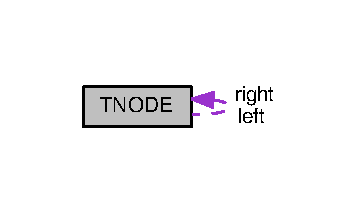
\includegraphics[width=172pt]{structTNODE__coll__graph}
\end{center}
\end{figure}
\subsubsection*{Public Member Functions}
\begin{DoxyCompactItemize}
\item 
\hyperlink{structTNODE_a0f2d73dc28ef3be182dbb07464560a47}{T\+N\+O\+D\+E} ()
\end{DoxyCompactItemize}
\subsubsection*{Public Attributes}
\begin{DoxyCompactItemize}
\item 
char \hyperlink{structTNODE_a436db20d992c4227b8482603b4f76712}{symbol}
\item 
\hyperlink{structTNODE}{T\+N\+O\+D\+E} $\ast$ \hyperlink{structTNODE_ac8548d0ee2d54b914e0e07ab35375dba}{left}
\item 
\hyperlink{structTNODE}{T\+N\+O\+D\+E} $\ast$ \hyperlink{structTNODE_a4e135d9137519b2a4b89dbccb55ae967}{right}
\end{DoxyCompactItemize}


\subsubsection{Constructor \& Destructor Documentation}
\hypertarget{structTNODE_a0f2d73dc28ef3be182dbb07464560a47}{\index{T\+N\+O\+D\+E@{T\+N\+O\+D\+E}!T\+N\+O\+D\+E@{T\+N\+O\+D\+E}}
\index{T\+N\+O\+D\+E@{T\+N\+O\+D\+E}!T\+N\+O\+D\+E@{T\+N\+O\+D\+E}}
\paragraph[{T\+N\+O\+D\+E}]{\setlength{\rightskip}{0pt plus 5cm}T\+N\+O\+D\+E\+::\+T\+N\+O\+D\+E (
\begin{DoxyParamCaption}
{}
\end{DoxyParamCaption}
)\hspace{0.3cm}{\ttfamily [inline]}}}\label{structTNODE_a0f2d73dc28ef3be182dbb07464560a47}

\begin{DoxyCode}
17             \{ \textcolor{comment}{// Constructor}
18         \hyperlink{structTNODE_a436db20d992c4227b8482603b4f76712}{symbol} = \textcolor{charliteral}{'*'};
19         \hyperlink{structTNODE_ac8548d0ee2d54b914e0e07ab35375dba}{left} = 0;
20         \hyperlink{structTNODE_a4e135d9137519b2a4b89dbccb55ae967}{right} = 0;
21     \}
\end{DoxyCode}


\subsubsection{Member Data Documentation}
\hypertarget{structTNODE_ac8548d0ee2d54b914e0e07ab35375dba}{\index{T\+N\+O\+D\+E@{T\+N\+O\+D\+E}!left@{left}}
\index{left@{left}!T\+N\+O\+D\+E@{T\+N\+O\+D\+E}}
\paragraph[{left}]{\setlength{\rightskip}{0pt plus 5cm}{\bf T\+N\+O\+D\+E}$\ast$ T\+N\+O\+D\+E\+::left}}\label{structTNODE_ac8548d0ee2d54b914e0e07ab35375dba}
\hypertarget{structTNODE_a4e135d9137519b2a4b89dbccb55ae967}{\index{T\+N\+O\+D\+E@{T\+N\+O\+D\+E}!right@{right}}
\index{right@{right}!T\+N\+O\+D\+E@{T\+N\+O\+D\+E}}
\paragraph[{right}]{\setlength{\rightskip}{0pt plus 5cm}{\bf T\+N\+O\+D\+E}$\ast$ T\+N\+O\+D\+E\+::right}}\label{structTNODE_a4e135d9137519b2a4b89dbccb55ae967}
\hypertarget{structTNODE_a436db20d992c4227b8482603b4f76712}{\index{T\+N\+O\+D\+E@{T\+N\+O\+D\+E}!symbol@{symbol}}
\index{symbol@{symbol}!T\+N\+O\+D\+E@{T\+N\+O\+D\+E}}
\paragraph[{symbol}]{\setlength{\rightskip}{0pt plus 5cm}char T\+N\+O\+D\+E\+::symbol}}\label{structTNODE_a436db20d992c4227b8482603b4f76712}


The documentation for this struct was generated from the following file\+:\begin{DoxyCompactItemize}
\item 
\hyperlink{morse_8h}{morse.\+h}\end{DoxyCompactItemize}

\hypertarget{structTREENODE}{\subsection{T\+R\+E\+E\+N\+O\+D\+E Struct Reference}
\label{structTREENODE}\index{T\+R\+E\+E\+N\+O\+D\+E@{T\+R\+E\+E\+N\+O\+D\+E}}
}


{\ttfamily \#include $<$tree.\+h$>$}



Collaboration diagram for T\+R\+E\+E\+N\+O\+D\+E\+:\nopagebreak
\begin{figure}[H]
\begin{center}
\leavevmode
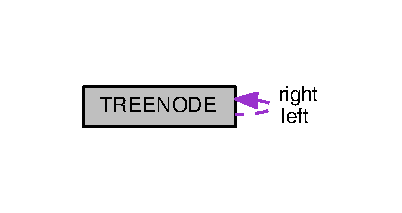
\includegraphics[width=193pt]{structTREENODE__coll__graph}
\end{center}
\end{figure}
\subsubsection*{Public Attributes}
\begin{DoxyCompactItemize}
\item 
S\+O\+M\+E\+T\+Y\+P\+E \hyperlink{structTREENODE_a16ae670d55c94f5358ae792a513e1e3c}{data}
\item 
\hyperlink{structTREENODE}{T\+R\+E\+E\+N\+O\+D\+E} $\ast$ \hyperlink{structTREENODE_a410b5b4e739703d7604d2bc7c5eddda9}{left}
\item 
\hyperlink{structTREENODE}{T\+R\+E\+E\+N\+O\+D\+E} $\ast$ \hyperlink{structTREENODE_a8b5bca93407a19121eefe5e0f08c4307}{right}
\end{DoxyCompactItemize}


\subsubsection{Member Data Documentation}
\hypertarget{structTREENODE_a16ae670d55c94f5358ae792a513e1e3c}{\index{T\+R\+E\+E\+N\+O\+D\+E@{T\+R\+E\+E\+N\+O\+D\+E}!data@{data}}
\index{data@{data}!T\+R\+E\+E\+N\+O\+D\+E@{T\+R\+E\+E\+N\+O\+D\+E}}
\paragraph[{data}]{\setlength{\rightskip}{0pt plus 5cm}S\+O\+M\+E\+T\+Y\+P\+E T\+R\+E\+E\+N\+O\+D\+E\+::data}}\label{structTREENODE_a16ae670d55c94f5358ae792a513e1e3c}
\hypertarget{structTREENODE_a410b5b4e739703d7604d2bc7c5eddda9}{\index{T\+R\+E\+E\+N\+O\+D\+E@{T\+R\+E\+E\+N\+O\+D\+E}!left@{left}}
\index{left@{left}!T\+R\+E\+E\+N\+O\+D\+E@{T\+R\+E\+E\+N\+O\+D\+E}}
\paragraph[{left}]{\setlength{\rightskip}{0pt plus 5cm}{\bf T\+R\+E\+E\+N\+O\+D\+E}$\ast$ T\+R\+E\+E\+N\+O\+D\+E\+::left}}\label{structTREENODE_a410b5b4e739703d7604d2bc7c5eddda9}
\hypertarget{structTREENODE_a8b5bca93407a19121eefe5e0f08c4307}{\index{T\+R\+E\+E\+N\+O\+D\+E@{T\+R\+E\+E\+N\+O\+D\+E}!right@{right}}
\index{right@{right}!T\+R\+E\+E\+N\+O\+D\+E@{T\+R\+E\+E\+N\+O\+D\+E}}
\paragraph[{right}]{\setlength{\rightskip}{0pt plus 5cm}{\bf T\+R\+E\+E\+N\+O\+D\+E}$\ast$ T\+R\+E\+E\+N\+O\+D\+E\+::right}}\label{structTREENODE_a8b5bca93407a19121eefe5e0f08c4307}


The documentation for this struct was generated from the following file\+:\begin{DoxyCompactItemize}
\item 
\hyperlink{tree_8h}{tree.\+h}\end{DoxyCompactItemize}

\section{File Documentation}
\hypertarget{lab_8dox}{\subsection{lab.\+dox File Reference}
\label{lab_8dox}\index{lab.\+dox@{lab.\+dox}}
}

\hypertarget{main_8cpp}{\subsection{main.\+cpp File Reference}
\label{main_8cpp}\index{main.\+cpp@{main.\+cpp}}
}
{\ttfamily \#include \char`\"{}lab.\+h\char`\"{}}\\*
Include dependency graph for main.\+cpp\+:\nopagebreak
\begin{figure}[H]
\begin{center}
\leavevmode
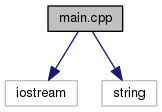
\includegraphics[width=350pt]{main_8cpp__incl}
\end{center}
\end{figure}
\subsubsection*{Functions}
\begin{DoxyCompactItemize}
\item 
int \hyperlink{main_8cpp_ae66f6b31b5ad750f1fe042a706a4e3d4}{main} ()
\end{DoxyCompactItemize}
\subsubsection*{Variables}
\begin{DoxyCompactItemize}
\item 
Fl\+\_\+\+Input $\ast$ \hyperlink{main_8cpp_abf805c82a90897837d1c26ef915f1cd6}{pizza}
\item 
Fl\+\_\+\+Output $\ast$ \hyperlink{main_8cpp_a05c7f6e86cca5f4d0ebf44d1f5042c37}{watch}
\item 
Fl\+\_\+\+Text\+\_\+\+Buffer $\ast$ \hyperlink{main_8cpp_aea2b8efadc87a819fe57c311d668e504}{buff}
\item 
Fl\+\_\+\+Text\+\_\+\+Display $\ast$ \hyperlink{main_8cpp_a23f917547a833922fd6bc8797cc04ee1}{order\+Q}
\end{DoxyCompactItemize}


\subsubsection{Function Documentation}
\hypertarget{main_8cpp_ae66f6b31b5ad750f1fe042a706a4e3d4}{\index{main.\+cpp@{main.\+cpp}!main@{main}}
\index{main@{main}!main.\+cpp@{main.\+cpp}}
\paragraph[{main}]{\setlength{\rightskip}{0pt plus 5cm}int main (
\begin{DoxyParamCaption}
{}
\end{DoxyParamCaption}
)}}\label{main_8cpp_ae66f6b31b5ad750f1fe042a706a4e3d4}

\begin{DoxyCode}
10 \{
11     Fl\_Cairo\_Window cw(400,300); \textcolor{comment}{// width & height of window}
12     cw.label(\textcolor{stringliteral}{"Pizza Deliveries Extravaganja"}); \textcolor{comment}{// title of your cairo window}
13     \textcolor{comment}{//cw.color(FL\_GREEN);}
14     
15     \hyperlink{main_8cpp_abf805c82a90897837d1c26ef915f1cd6}{pizza} = \textcolor{keyword}{new} Fl\_Input(190, 20, 100, 20, \textcolor{stringliteral}{"pizza:"});
16     \hyperlink{main_8cpp_abf805c82a90897837d1c26ef915f1cd6}{pizza}->labelcolor(FL\_BLUE);
17     
18     \hyperlink{main_8cpp_aea2b8efadc87a819fe57c311d668e504}{buff} = \textcolor{keyword}{new} Fl\_Text\_Buffer();
19     \hyperlink{main_8cpp_a23f917547a833922fd6bc8797cc04ee1}{orderQ} = \textcolor{keyword}{new} Fl\_Text\_Display(100,100,100,100,\textcolor{stringliteral}{"Order Q"});
20     \hyperlink{main_8cpp_a23f917547a833922fd6bc8797cc04ee1}{orderQ}->buffer(\hyperlink{main_8cpp_aea2b8efadc87a819fe57c311d668e504}{buff});
21     
22     \hyperlink{main_8cpp_a05c7f6e86cca5f4d0ebf44d1f5042c37}{watch} = \textcolor{keyword}{new} Fl\_Output(70,20,50,20,\textcolor{stringliteral}{"seconds:"});
23     
24     Fl\_Button b(330, 60, 50, 20, \textcolor{stringliteral}{"Order:"});
25     b.callback((Fl\_Callback*)\hyperlink{lab_8h_a547f84331a8c529348e1130ca169c69c}{order\_cb});
26     
27     cw.show();
28     Fl::add\_timeout(1,\hyperlink{lab_8h_a13ed8751dfa95731ad8930762493b16b}{timer});
29     \textcolor{keywordflow}{return} Fl::run();
30 \}
\end{DoxyCode}


\subsubsection{Variable Documentation}
\hypertarget{main_8cpp_aea2b8efadc87a819fe57c311d668e504}{\index{main.\+cpp@{main.\+cpp}!buff@{buff}}
\index{buff@{buff}!main.\+cpp@{main.\+cpp}}
\paragraph[{buff}]{\setlength{\rightskip}{0pt plus 5cm}Fl\+\_\+\+Text\+\_\+\+Buffer$\ast$ buff}}\label{main_8cpp_aea2b8efadc87a819fe57c311d668e504}
\hypertarget{main_8cpp_a23f917547a833922fd6bc8797cc04ee1}{\index{main.\+cpp@{main.\+cpp}!order\+Q@{order\+Q}}
\index{order\+Q@{order\+Q}!main.\+cpp@{main.\+cpp}}
\paragraph[{order\+Q}]{\setlength{\rightskip}{0pt plus 5cm}Fl\+\_\+\+Text\+\_\+\+Display$\ast$ order\+Q}}\label{main_8cpp_a23f917547a833922fd6bc8797cc04ee1}
\hypertarget{main_8cpp_abf805c82a90897837d1c26ef915f1cd6}{\index{main.\+cpp@{main.\+cpp}!pizza@{pizza}}
\index{pizza@{pizza}!main.\+cpp@{main.\+cpp}}
\paragraph[{pizza}]{\setlength{\rightskip}{0pt plus 5cm}Fl\+\_\+\+Input$\ast$ pizza}}\label{main_8cpp_abf805c82a90897837d1c26ef915f1cd6}
\hypertarget{main_8cpp_a05c7f6e86cca5f4d0ebf44d1f5042c37}{\index{main.\+cpp@{main.\+cpp}!watch@{watch}}
\index{watch@{watch}!main.\+cpp@{main.\+cpp}}
\paragraph[{watch}]{\setlength{\rightskip}{0pt plus 5cm}Fl\+\_\+\+Output$\ast$ watch}}\label{main_8cpp_a05c7f6e86cca5f4d0ebf44d1f5042c37}

\hypertarget{morse_8cpp}{\subsection{morse.\+cpp File Reference}
\label{morse_8cpp}\index{morse.\+cpp@{morse.\+cpp}}
}
{\ttfamily \#include \char`\"{}morse.\+h\char`\"{}}\\*

\hypertarget{morse_8dox}{\subsection{morse.\+dox File Reference}
\label{morse_8dox}\index{morse.\+dox@{morse.\+dox}}
}

\hypertarget{morse_8h}{\subsection{morse.\+h File Reference}
\label{morse_8h}\index{morse.\+h@{morse.\+h}}
}
{\ttfamily \#include $<$iostream$>$}\\*
{\ttfamily \#include $<$cctype$>$}\\*
{\ttfamily \#include $<$string.\+h$>$}\\*
\subsubsection*{Classes}
\begin{DoxyCompactItemize}
\item 
struct \hyperlink{structMorsecode}{Morsecode}
\item 
struct \hyperlink{structTNODE}{T\+N\+O\+D\+E}
\item 
class \hyperlink{classTelegraph}{Telegraph}
\end{DoxyCompactItemize}

\hypertarget{morseCode_8h}{\subsection{morse\+Code.\+h File Reference}
\label{morseCode_8h}\index{morse\+Code.\+h@{morse\+Code.\+h}}
}
\subsubsection*{Variables}
\begin{DoxyCompactItemize}
\item 
\hyperlink{structMorsecode}{Morsecode} \hyperlink{morseCode_8h_a2014b8783fa4dd5ed737143bf3dbaf68}{table} \mbox{[}$\,$\mbox{]}
\end{DoxyCompactItemize}


\subsubsection{Variable Documentation}
\hypertarget{morseCode_8h_a2014b8783fa4dd5ed737143bf3dbaf68}{\index{morse\+Code.\+h@{morse\+Code.\+h}!table@{table}}
\index{table@{table}!morse\+Code.\+h@{morse\+Code.\+h}}
\paragraph[{table}]{\setlength{\rightskip}{0pt plus 5cm}{\bf Morsecode} table\mbox{[}$\,$\mbox{]}}}\label{morseCode_8h_a2014b8783fa4dd5ed737143bf3dbaf68}
{\bfseries Initial value\+:}
\begin{DoxyCode}
= \{
  \{\textcolor{charliteral}{'A'}, \textcolor{stringliteral}{".-"}\},     \{\textcolor{charliteral}{'B'}, \textcolor{stringliteral}{"-..."}\},    \{\textcolor{charliteral}{'C'}, \textcolor{stringliteral}{"-.-."}\},   \{\textcolor{charliteral}{'D'}, \textcolor{stringliteral}{"-.."}\},
  \{\textcolor{charliteral}{'E'}, \textcolor{stringliteral}{"."}\},      \{\textcolor{charliteral}{'F'}, \textcolor{stringliteral}{"..-."}\},    \{\textcolor{charliteral}{'G'}, \textcolor{stringliteral}{"--."}\},    \{\textcolor{charliteral}{'H'}, \textcolor{stringliteral}{"...."}\},
  \{\textcolor{charliteral}{'I'}, \textcolor{stringliteral}{".."}\},     \{\textcolor{charliteral}{'J'}, \textcolor{stringliteral}{".---"}\},    \{\textcolor{charliteral}{'K'}, \textcolor{stringliteral}{"-.-"}\},    \{\textcolor{charliteral}{'L'}, \textcolor{stringliteral}{".-.."}\},
  \{\textcolor{charliteral}{'M'}, \textcolor{stringliteral}{"--"}\},     \{\textcolor{charliteral}{'N'}, \textcolor{stringliteral}{"-."}\},      \{\textcolor{charliteral}{'O'}, \textcolor{stringliteral}{"---"}\},    \{\textcolor{charliteral}{'P'}, \textcolor{stringliteral}{".--."}\},
  \{\textcolor{charliteral}{'Q'}, \textcolor{stringliteral}{"--.-"}\},   \{\textcolor{charliteral}{'R'}, \textcolor{stringliteral}{".-."}\},     \{\textcolor{charliteral}{'S'}, \textcolor{stringliteral}{"..."}\},    \{\textcolor{charliteral}{'T'}, \textcolor{stringliteral}{"-"}\},
  \{\textcolor{charliteral}{'U'}, \textcolor{stringliteral}{"..-"}\},    \{\textcolor{charliteral}{'V'}, \textcolor{stringliteral}{"...-"}\},    \{\textcolor{charliteral}{'W'}, \textcolor{stringliteral}{".--"}\},    \{\textcolor{charliteral}{'X'}, \textcolor{stringliteral}{"-..-"}\},
  \{\textcolor{charliteral}{'Y'}, \textcolor{stringliteral}{"-.--"}\},   \{\textcolor{charliteral}{'Z'}, \textcolor{stringliteral}{"--.."}\},
  \{\textcolor{charliteral}{'0'}, \textcolor{stringliteral}{"-----"}\},  \{\textcolor{charliteral}{'1'}, \textcolor{stringliteral}{".----"}\},   \{\textcolor{charliteral}{'2'}, \textcolor{stringliteral}{"..---"}\},  \{\textcolor{charliteral}{'3'}, \textcolor{stringliteral}{"...--"}\},
  \{\textcolor{charliteral}{'4'}, \textcolor{stringliteral}{"....-"}\},  \{\textcolor{charliteral}{'5'}, \textcolor{stringliteral}{"....."}\},   \{\textcolor{charliteral}{'6'}, \textcolor{stringliteral}{"-...."}\},  \{\textcolor{charliteral}{'7'}, \textcolor{stringliteral}{"--..."}\},
  \{\textcolor{charliteral}{'8'}, \textcolor{stringliteral}{"---.."}\},  \{\textcolor{charliteral}{'9'}, \textcolor{stringliteral}{"----."}\},
  \{\textcolor{charliteral}{'.'}, \textcolor{stringliteral}{".-.-.-"}\}, \{\textcolor{charliteral}{','}, \textcolor{stringliteral}{"--..--"}\},  \{\textcolor{charliteral}{'?'}, \textcolor{stringliteral}{"..--.."}\},
  \{\textcolor{charliteral}{'\(\backslash\)0'}, \textcolor{stringliteral}{""}\}
\}
\end{DoxyCode}

\hypertarget{tree_8h}{\subsection{tree.\+h File Reference}
\label{tree_8h}\index{tree.\+h@{tree.\+h}}
}
\subsubsection*{Classes}
\begin{DoxyCompactItemize}
\item 
struct \hyperlink{structTREENODE}{T\+R\+E\+E\+N\+O\+D\+E}
\end{DoxyCompactItemize}
\subsubsection*{Functions}
\begin{DoxyCompactItemize}
\item 
void \hyperlink{tree_8h_a392480642e3e93f0ab75f03aa20c0ac9}{Destroy} (\hyperlink{structTREENODE}{T\+R\+E\+E\+N\+O\+D\+E} $\ast$root)
\item 
int \hyperlink{tree_8h_abeb540f2c3d07690ac75469989c3068a}{Compare} (const S\+O\+M\+E\+T\+Y\+P\+E data1, const S\+O\+M\+E\+T\+Y\+P\+E data2)
\item 
void \hyperlink{tree_8h_a2e1a42346c44f631e51044afec676c22}{Copy} (const S\+O\+M\+E\+T\+Y\+P\+E data1, S\+O\+M\+E\+T\+Y\+P\+E data2)
\end{DoxyCompactItemize}


\subsubsection{Function Documentation}
\hypertarget{tree_8h_abeb540f2c3d07690ac75469989c3068a}{\index{tree.\+h@{tree.\+h}!Compare@{Compare}}
\index{Compare@{Compare}!tree.\+h@{tree.\+h}}
\paragraph[{Compare}]{\setlength{\rightskip}{0pt plus 5cm}int Compare (
\begin{DoxyParamCaption}
\item[{const S\+O\+M\+E\+T\+Y\+P\+E}]{data1, }
\item[{const S\+O\+M\+E\+T\+Y\+P\+E}]{data2}
\end{DoxyParamCaption}
)}}\label{tree_8h_abeb540f2c3d07690ac75469989c3068a}
\hypertarget{tree_8h_a2e1a42346c44f631e51044afec676c22}{\index{tree.\+h@{tree.\+h}!Copy@{Copy}}
\index{Copy@{Copy}!tree.\+h@{tree.\+h}}
\paragraph[{Copy}]{\setlength{\rightskip}{0pt plus 5cm}void Copy (
\begin{DoxyParamCaption}
\item[{const S\+O\+M\+E\+T\+Y\+P\+E}]{data1, }
\item[{S\+O\+M\+E\+T\+Y\+P\+E}]{data2}
\end{DoxyParamCaption}
)}}\label{tree_8h_a2e1a42346c44f631e51044afec676c22}
\hypertarget{tree_8h_a392480642e3e93f0ab75f03aa20c0ac9}{\index{tree.\+h@{tree.\+h}!Destroy@{Destroy}}
\index{Destroy@{Destroy}!tree.\+h@{tree.\+h}}
\paragraph[{Destroy}]{\setlength{\rightskip}{0pt plus 5cm}void Destroy (
\begin{DoxyParamCaption}
\item[{{\bf T\+R\+E\+E\+N\+O\+D\+E} $\ast$}]{root}
\end{DoxyParamCaption}
)}}\label{tree_8h_a392480642e3e93f0ab75f03aa20c0ac9}

%--- End generated contents ---

% Index
\newpage
\phantomsection
\addcontentsline{toc}{section}{Index}
\printindex

\end{document}
